\chapter{Clase 4. Exposición de los problemas de la clase 3}
\textbf{18/02/2025}

Se formaron distintos equipos a la clase anterior y en algunos casos se plantearon resoluciones distintas a las que se habían llegado anteriormente, tanto en el equipo en el que me encontraba como en los que expusieron los demás problemas. 

Solo en los casos en los que se planteó una solución diferente a la que se llegó en la clase anterior serán mencionados, por lo tanto se podrá consultar la sección \hyperref[sec:C3ACERTIJOS]{acertijos} para ver las demás resoluciones.

\section{Problema 1}
\begin{figure}[h!]
    \begin{center}
        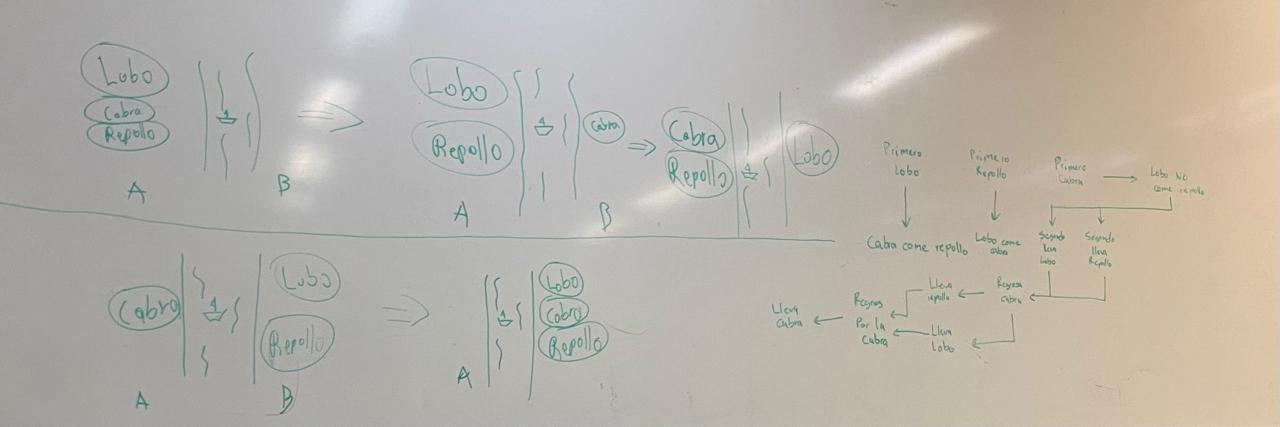
\includegraphics[scale=0.2]{clase4/problema1.jpeg}
    \end{center}
    \caption{Resolución al problema 2}
\end{figure}

\section{Problema 2}
La primera solución que plantearon fue la misma que a \hyperref[ejem:c3P2]{la anterior clase}, donde proponían romper cada trozo de cadena y lo representaron como una suma, pero luego utilizando el mismo método decidieron poner solo cuatro números 3 y cada signo mas representaría el quinto trozo de cadena, de este modo llegaron a la conclusión de que la cantidad mínima de eslabones a romper sería de 3.
\begin{figure}[h!]
    \begin{center}
        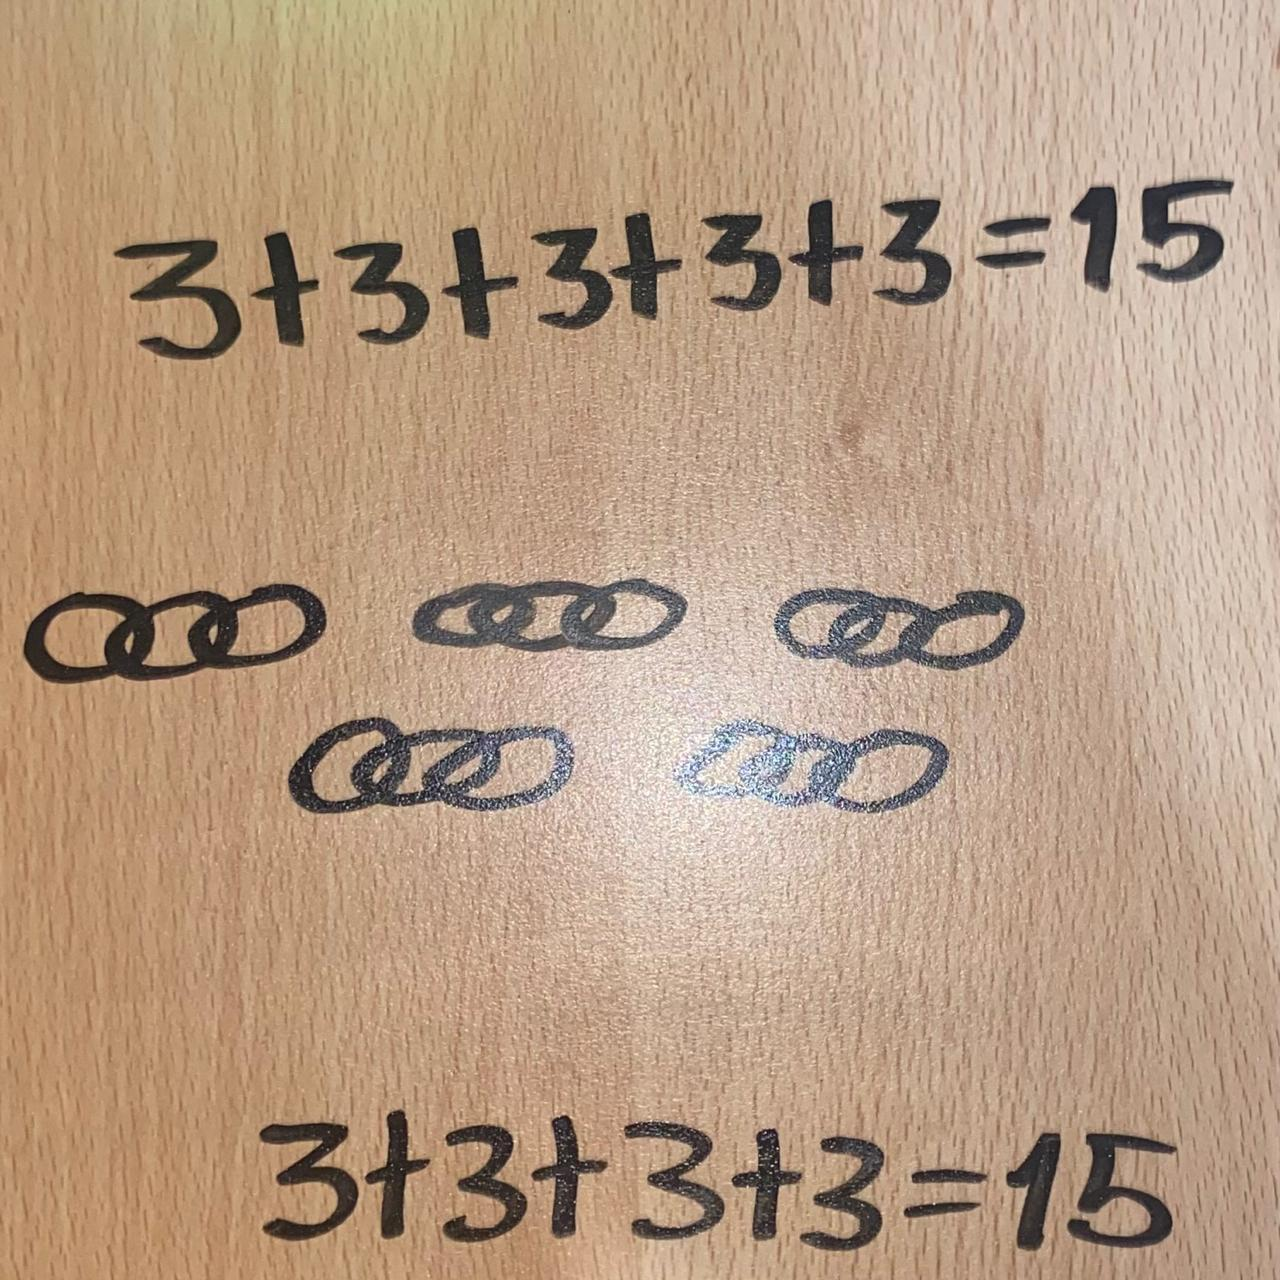
\includegraphics[scale=0.09]{clase4/problema2.jpeg}
    \end{center}
    \caption{Resolución al problema 2}
\end{figure}

\section{Problema 3}
\begin{figure}[h!]
    \begin{center}
        \begin{tabular}{cc}
            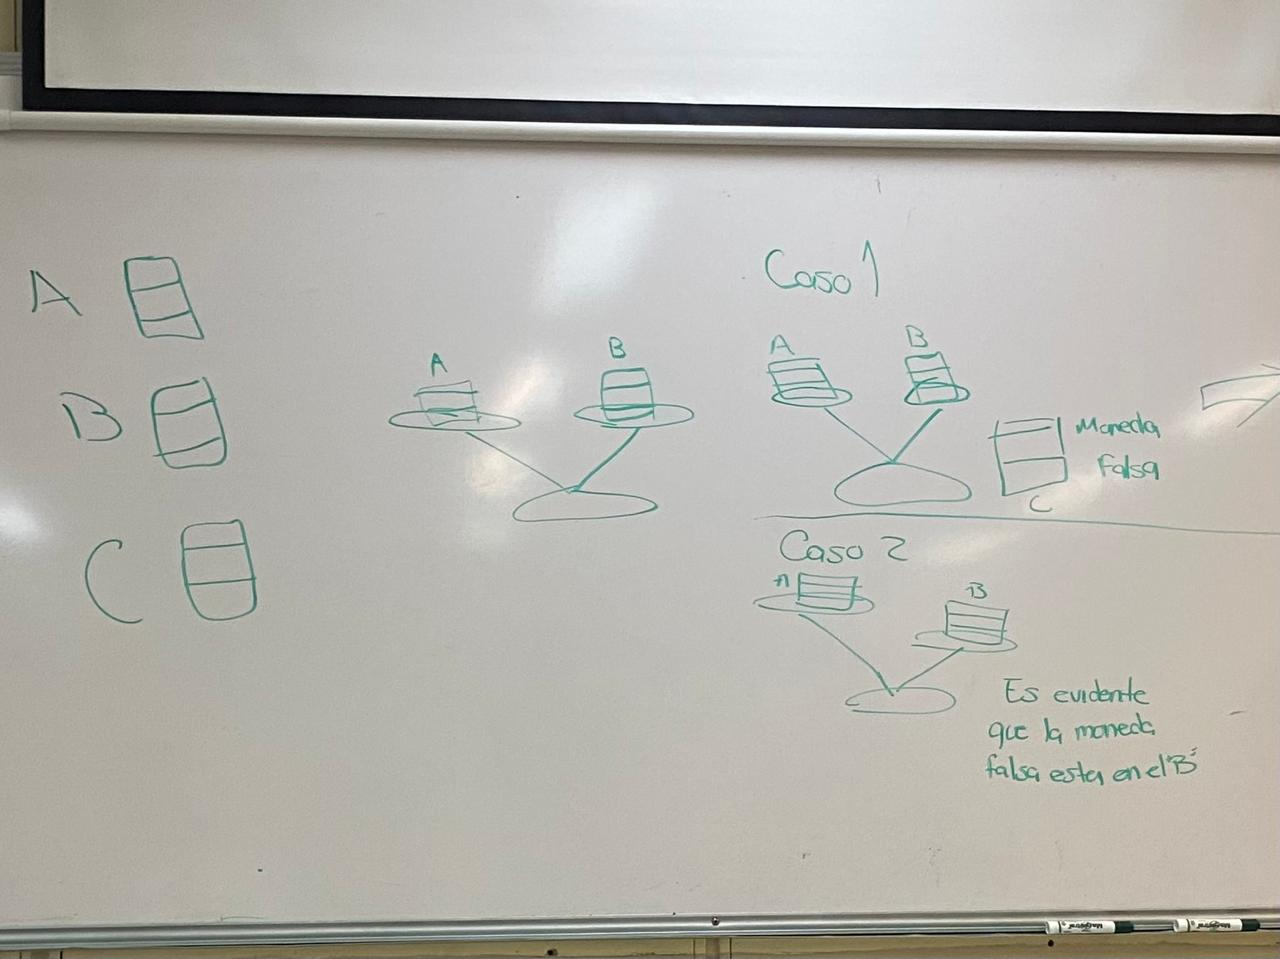
\includegraphics[scale=0.15]{clase4/problema3.1.jpeg}&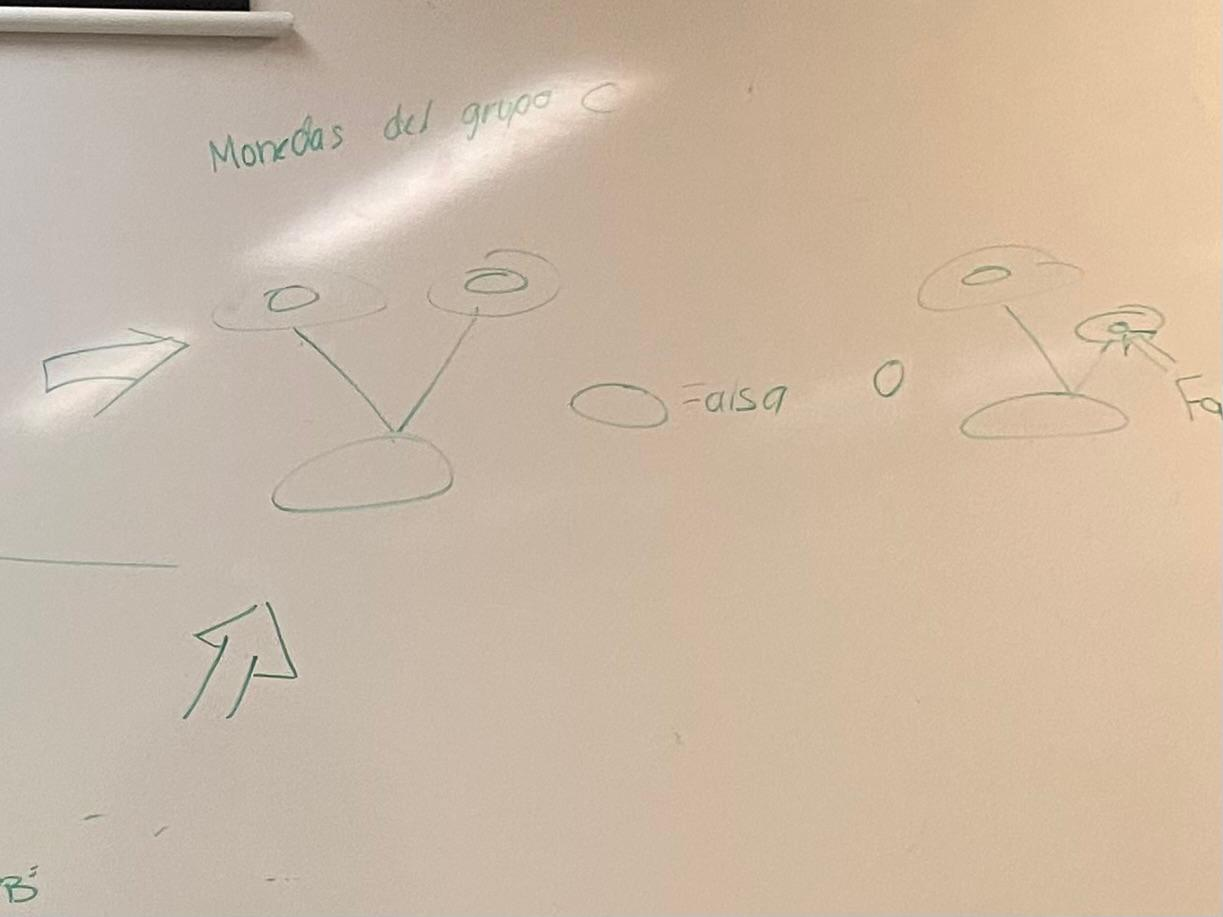
\includegraphics[scale=0.15]{clase4/problema3.2.jpeg}
        \end{tabular}
    \end{center}
    \caption{Resoluciónal al problema 3}
\end{figure}

\section{Problema 4}
La segunda solución la propuso un equipo diferente al que estaba exponiendo, pues el segundo caso que observaron los expositores, lo descartaron y otro equipo, y sólo la observación siguiente:
Después de llenar la jarra de 5 l, se pasaba 3 l a la jarra más pequeña y se descartaban, mientras que en la jarra más grande quedaban 2 l los cuales nuevamente se pasaban a la jarra más chica y por última vez se llenaba la jarra de cinco y se vertía 1 l en la jarra de tres, quedando así 4 l en la jarra más grande. Este es un caso similar al planteado en la anterior clase.

\begin{figure}[h!]
    \caption{Resolución al problema 4}
    \begin{center}
        \begin{tabular}{cccc}
            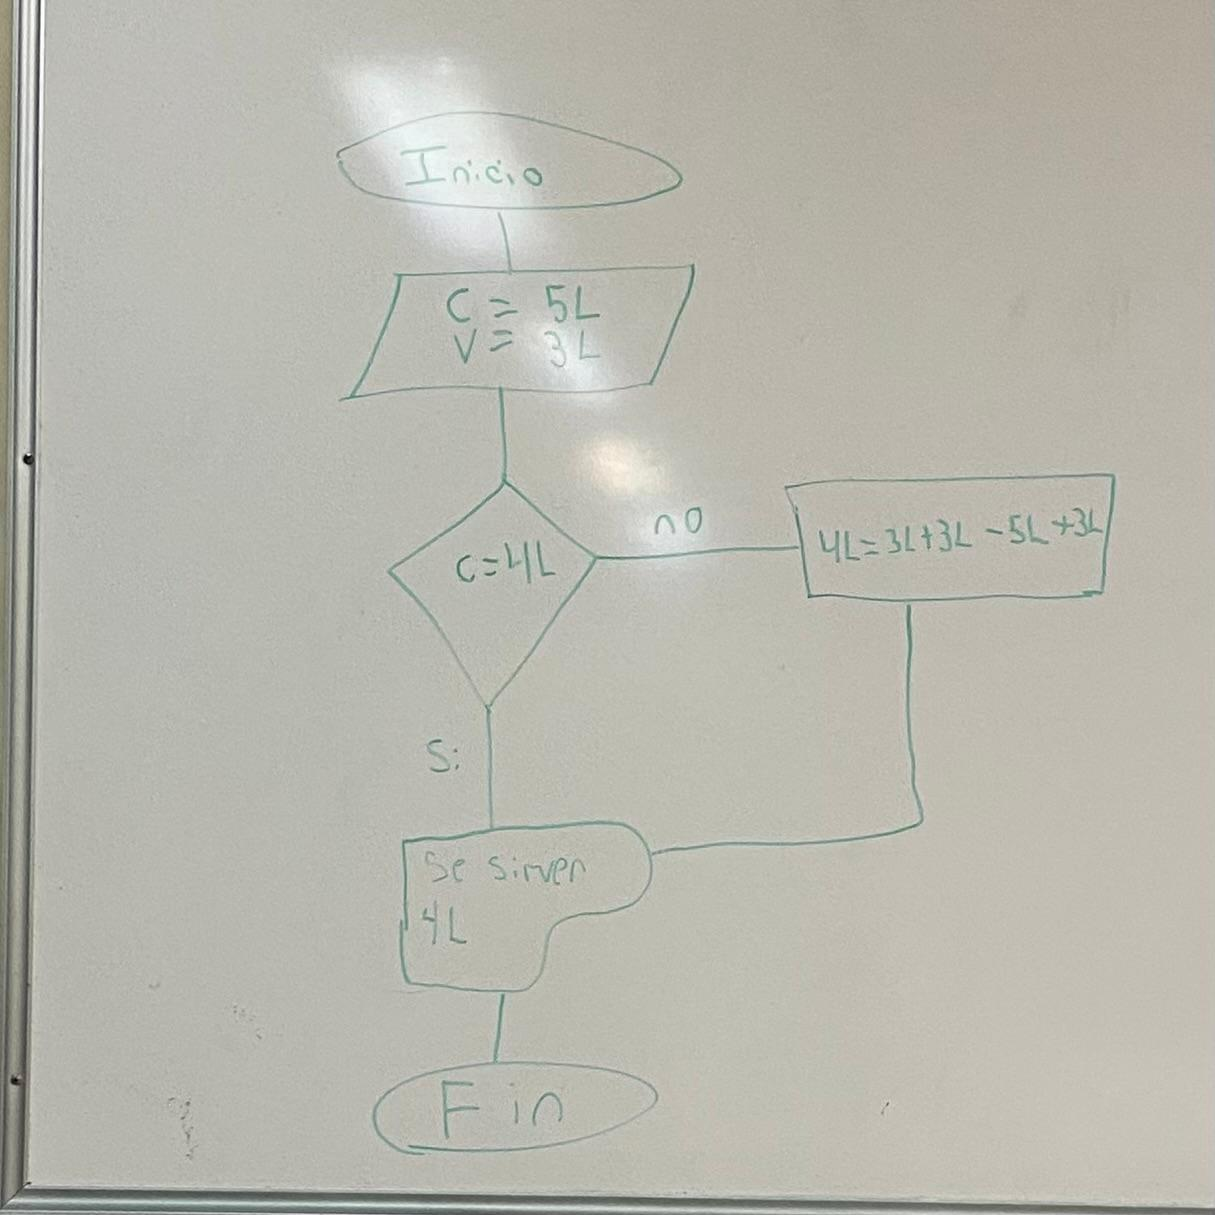
\includegraphics[scale=0.09]{clase4/problema4.1.jpeg}&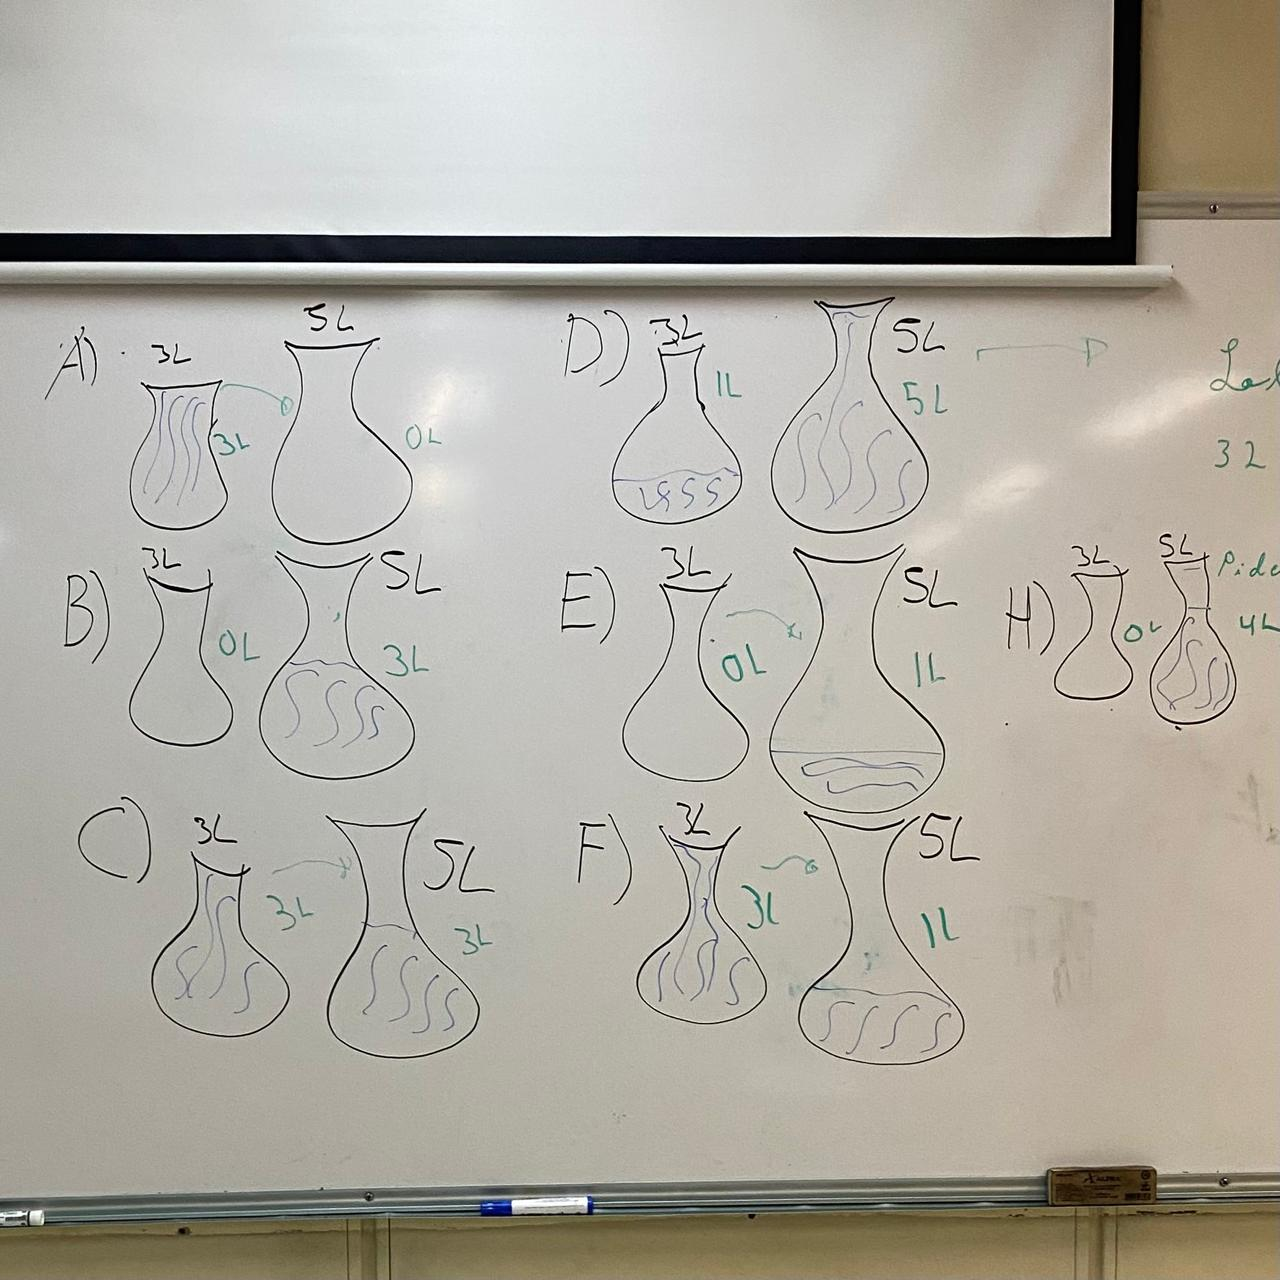
\includegraphics[scale=0.09]{clase4/problema4.2.jpeg}&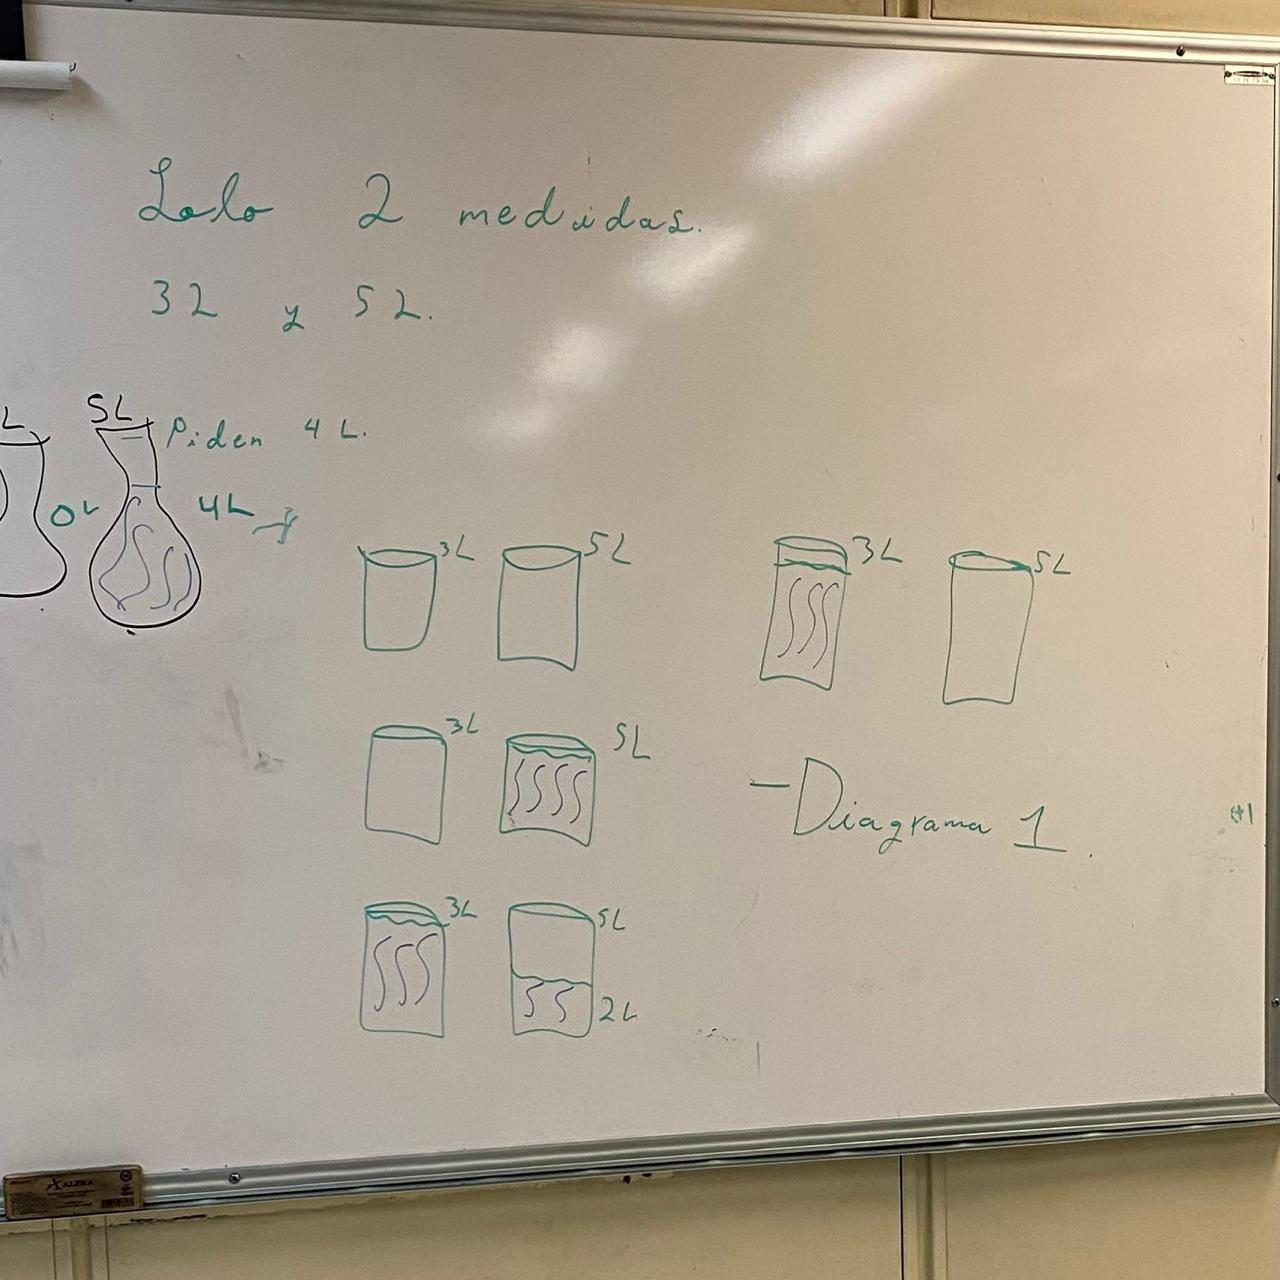
\includegraphics[scale=0.09]{clase4/problema4.3.jpeg}&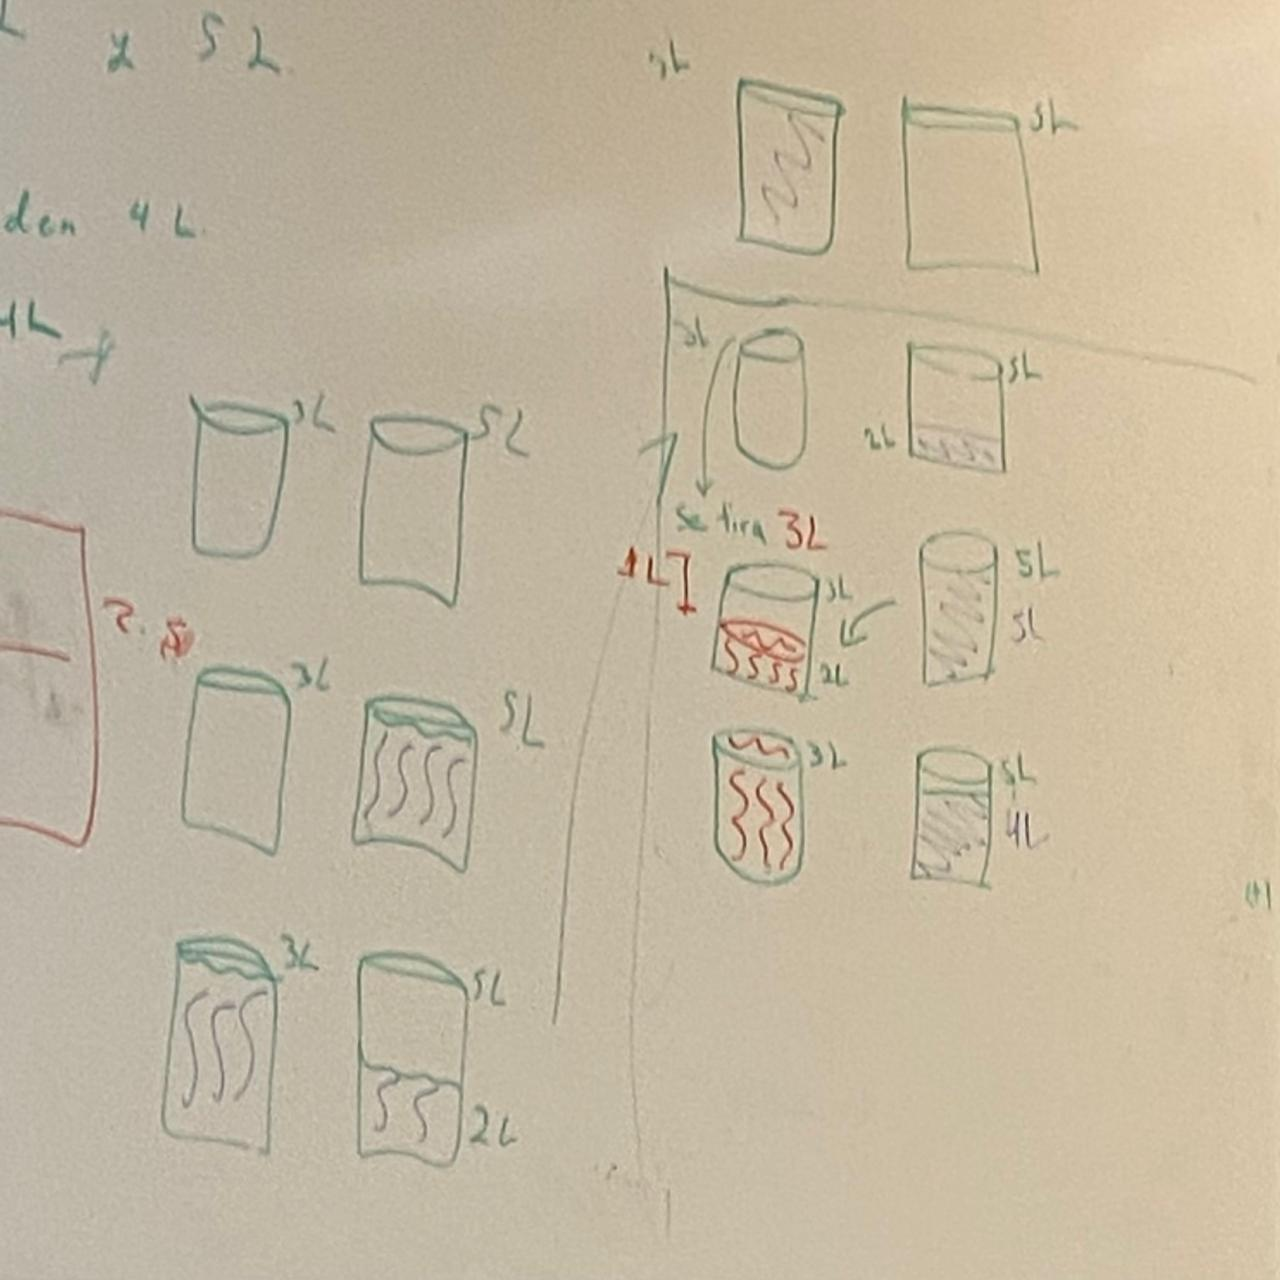
\includegraphics[scale=0.09]{clase4/problema4.4.jpeg}
        \end{tabular}
    \end{center}
\end{figure}

\section{Problema 5}
Fui parte del equipo que expuso la solución a este problema y se mencionaron las soluciones de la \hyperref[ejem:c3P5]{clase anterior}.
